\chapter{Detailed Description}
\section{Interpreter}
\subsection{Introduction}
The interpreter is a complete implementation of an interpreter for the \mmc language. It accepts input from the parser in the form of an AST (\emph{Abstract Syntax Tree}) and obeys the instructions contained within the nodes of the tree. We call the tree traversal ``a tree walk" and we use this walk to interpret \verb!NODE! terms on the fly. We will see this kind of recursive pattern several times throughout the whole project.
\subsection{Initial Scan}
Firstly, the interpreter scans the AST, looking for global variables and function definitions. This initial scan is done, as we have no idea where to start interpreting without the presence of some kind of entry point into the user's code. It was decided that the most sensible approach would be to require the user-supplied definition of an \verb!int main(void)! entry-point function, in a similar vain to C. As this initial sweep of the AST takes place, any global variables or function declarations are entered into a structure known as the ``environment". 
\ \\ \ \\
Another benefit of performing this initial scan, is that as all outermost functions (and global variables) will now be entered into the environment. This means that functions may call other outer-level functions regardless of the order of definition (i.e if one function calls one which is declared lower down in the file). The same, however, does not apply to inner functions / variables.
\subsection{Environment}
Quite simply, the environment houses everything that the interpreter considers to be in local scope at a given execution point. As such, after our initial scan, we can detect the presence of a valid entry-point function by examining the environment. This initial environment is known as the ``global environment", as everything contained within, is visible to the whole user program. This initial scan follows exactly the same code-path as the full interpreter does, but passes a flag, in order to ensure that function bodies are never stepped into.
\ \\ \ \\
The environment (depicted in figure \ref{fig:environment}) is a hash-table of \verb!values!. These values are references to inner functions or local variables. By following the static link between one environment and another (please see figure \ref{fig:environment}), it is possible to access and refer to values residing in outer scopes. The idea of a static link was given to us in relation to their use in Activation Records (please see section \ref{sec:MIPS}) during lectures. Different information is stored for functions as opposed to variables. The \verb!value!'s type is determined with the following constants, the main types are given here, although there are some used for other purposes that are not mentioned here for the sake of clarity.

\begin{description}
	\item[VT\_INTEGR] Values of this type are integer variables, integer constants or integer temporaries.
	\item[VT\_STRING] Strings cannot be stored in the environment (this language does not have a string type), this value type is used to construct temporary strings that can be passed around within the interpreter / compiler. Such string values are created when identifiers are walked over, for instance.
	\item[VT\_FUNCTN] These values represent pointers to functions. This can be either a function variable or an actual function.
\end{description}

\subsection{Invoking the Entry Point}
If no entry point is found, a fatal error is raised as interpretation cannot continue without a valid entry point. If the entry point was found in our global environment, we lookup where the function definition was found in the AST and execute from this point. The \verb!environment.c! file gives us lots of useful search functionality in order to do things such as this. The particular search we do to find the main entry point is to look for a function in the global environment called \verb!main! with an integer return type and no formal parameters. If we get a match, we are returned a \verb!value! structure (of type \verb!VT_FUNCTN!) which meets our requirements within the global environment. These ``function values" each hold a reference to what \verb!NODE! in the AST is considered the ``start of the function". Once we have found the corresponding ``start of function" \verb!NODE! for the \verb!main()! function, we are able to continue the interpretation process by calling \verb!evaluate! on this entry \verb!NODE!.

\subsection{Recursive function - evaluate()}
The \verb!evaluate! function is now called recursively starting from the entry point. This scan is different from the initial scan, because we now look inside function bodies and any nested functions contained therein. Every time we enter a new function or block (such as an \emph{if statement} or \emph{while loop}), a new environment is created with a static link to the environment of the parent (enclosing) function (or the global environment, as appropriate). As we step over the tree in this recursive function, we encounter \verb!NODES! that are present in the AST. The following list mentions the steps that are taken for the several different (more interesting) types of node. The terms LHS and RHS refer to the \emph{left-hand side} and \emph{right-hand side} of an expression respectively. As the AST is a binary tree, the LHS and RHS can be thought of as the two child nodes under the current node. Please see figure \ref{fig:ast} for an example AST, that will use some of the elements mentioned below.

\begin{description}
	\item[Arithmetic Operator] We look at the LHS and RHS of the expression call \verb!evaluate! recursively on each. We do this, to try and simplify both sides (operands) into integers. From each recursive call we get back a \verb!value! typed struct for each, which should now contain our simplified integer. If one side happened to be a function application, for instance, the recursive call has already made the necessary calls to coerce this into the appropriate integer value. We calculate the result of the arithmetic expression and return the calculated value.
	\item[= Operator] This is the assignment operator. We call \verb!evaluate! on the LHS to get the variable into which the result will be stored. For the assignment to be valid, we must have already defined the assignment variable in the environment. Otherwise, we would be  using a variable that has not been declared yet. We call \verb!evaluate! on the RHS to find out the value that we're trying to assign to the variable on the LHS. Once we have the value back, we \textbf{type check} the assignment to ensure that the assignment is valid. This prevents the user making mistakes like trying to assign an integer to a function typed variable. The type checking operation is a simple check on the \verb!value! type on the LHS and RHS to check that they match. If the types do not match, then a fatal error describing the problem is raised. If all checks pass, then the existing LHS variable is updated with the new RHS value. This assignment will always affect the variable in the environment of its definition. The next time this LHS variable is referenced, it will have the newly assigned value.
	\item[APPLY] The \verb!APPLY! node type is encountered when a function call will occur. On the LHS of an \verb!APPLY! node is the function name identifier and the RHS contains the list of parameters that are being passed to the function. To invoke the function, the function name is searched for within the current environment (traversing static links where necessary). If a function typed variable is provided instead of a function application, this function variable holds enough information for us to invoke the function without having to traverse multiple levels of environment. If the function is \emph{still} not found, a fatal interpreter error is raised. If the function is found, we switch to the function's definition environment. In this environment, we store new variables with the formal parameter names, but with the specified parameter values used when calling the function. This assignment is also type checked with precisely the same method as before (see point ``\textbf{= Operator}" above). Once the checks are complete, we now pass the AST node representing the start of the function body to the \verb!evaluate! function and wait for control to return with the associated return value.
	\item[WHILE] While loops are also possible in \mmc. The implementation for a \verb!WHILE! statement within \mmc relies on the \verb!while! construct in the host development language (C). Inside the condition for the while loop, we recursively call \verb!evaluate! on the user specified condition. The condition is on the LHS of the \verb!WHILE! statement. In the body of our while loop, we call \verb!evaluate! on the RHS, which is the body of the user supplied while loop. The return value of the RHS evaluation is checked for several special cases. If we are returned the special \verb!$BREAK! or \verb!$CONTINUE! values then we \verb!break!, or \verb!continue! by using the  corresponding C keywords. If any other value is returned, we immediately exit the loop and return this value.
	\item[IF and ELSE] The \verb!IF! statement is fairly similar to the \verb!WHILE! statement in that the LHS holds the branch condition and we use C's \verb!IF! statement to implement it. Obviously the condition is only considered once in an \verb!IF! statement. One added complication with an if statement, is that an \verb!IF! can be followed by an \verb!ELSE! node. An \verb!ELSE! node needs access to the result of the \verb!IF! condition in order to decide whether to branch to the true or false part of the \verb!ELSE! (please see figure \ref{fig:if} for a graphical example). To get around this problem, when the condition is evaluated in the \verb!IF!, the result of that condition is placed into the environment as a temporary integer called \verb!$IF!. When the \verb!ELSE! statement executes, it checks the value of \verb!$IF! to see whether it should branch left or right.
	\item[Functions] Function definitions span multiple nodes in a tree, because of the amount of information that a function signature contains. Starting from higher up in the AST, we see nodes \verb!D, d, F!. The way each of these nodes is handled is mentioned below.
		\begin{description}
			\item[D] On the LHS is the \verb!d! node (explained below). On the RHS is the function body, i.e. the first instruction that constitutes the start of the used-defined function. Once we have evaluated \verb!d!, we store the returned value in the current environment along with a \textbf{reference} to the start of the function body. \verb!evaluate! is not called on the RHS, because this is only done when the function is called. The value returned by \verb!d! is a complete function definition that provides enough information for the declared function to be executed.
			\item[d] On the LHS is the return type of the function, this can be \verb!VOID, INT,! or \verb!FUNCTION!. We add the return type of the function into the temporary function variable returned by the \verb!F! node on the RHS. This is passed back up to the \verb!D! node ready to be stored in the environment.
			\item[F] On the LHS is the function name (identifier). On the RHS is the list of formal parameters. The interpreter calls \verb!evaluate! on the RHS with a special flag to denote any variables found as parameters, rather than normal variables. This call will return a linked list of \verb!value! structures which contains the parameter list. Once we have the function name and parameters, we build a temporary \verb!VT_FUNCTN value! structure, which will be gradually augmented with information as it is passed up to the \verb!D! node.
		\end{description}
	\item[RETURN] The value to return is found on the LHS of the \verb!RETURN! statement. \verb!evaluate! is called on the node to simplify arithmetic operations or the result of another function call. If the value to return is an identifier (i.e. a variable or a function ptr) then this is looked up in the environment and this \verb!value! (if found) is returned instead of the identifier. Additionally, we also type  check the return value by comparing the current function's return type to the value type of the evaluated return value. If the types match then the appropriate value is returned, otherwise a fatal error is raised. The same process prevents us returning \verb!NULL!, when a return value is expected (based on the function definition having a non-\verb!VOID! return type). \textbf{Please note:} there is no check to ensure that we actually use a return statement at all, where one is expected, only that - if we do use a return statement, it is type-checked.
\end{description}

\subsection{Returning from main()}
After traversing the AST, the \verb!main! function should have a valid integer return value (unless no \verb!RETURN! statement was present). This value is simply printed to standard out and the interpreter finishes.

\subsection{State of the Interpreter}
Within the limited time that we had for the whole project and the testing completed as part of this, the interpreter is seemingly complete. It is capable of executing all of the example scripts that I have created and there are no significant faults that I know of. There are two known faults that can be mentioned briefly.
\begin{itemize}
	\item One thing that does not work in the interpreter, but parses correctly: Functions without parameters that use the keyword \verb!void! to denote no parameters: \verb!int my_parameterless_fn(void)!.
	\item Return values are type-checked, but no effort is made to detect functions that do not return a value, when they should.
\end{itemize}

\subsection{Testing}
To test the interpreter I wrote a small regression testing framework called \verb!bungee!\footnote{\url{http://github.com/henrythacker/bungee}}. After every change the script was fired off to ensure that all tests continue to yield the correct results. Unfortunately it will not run on the BUCS machines because certain Ruby dependencies are unavailable.

\begin{figure}[p]
	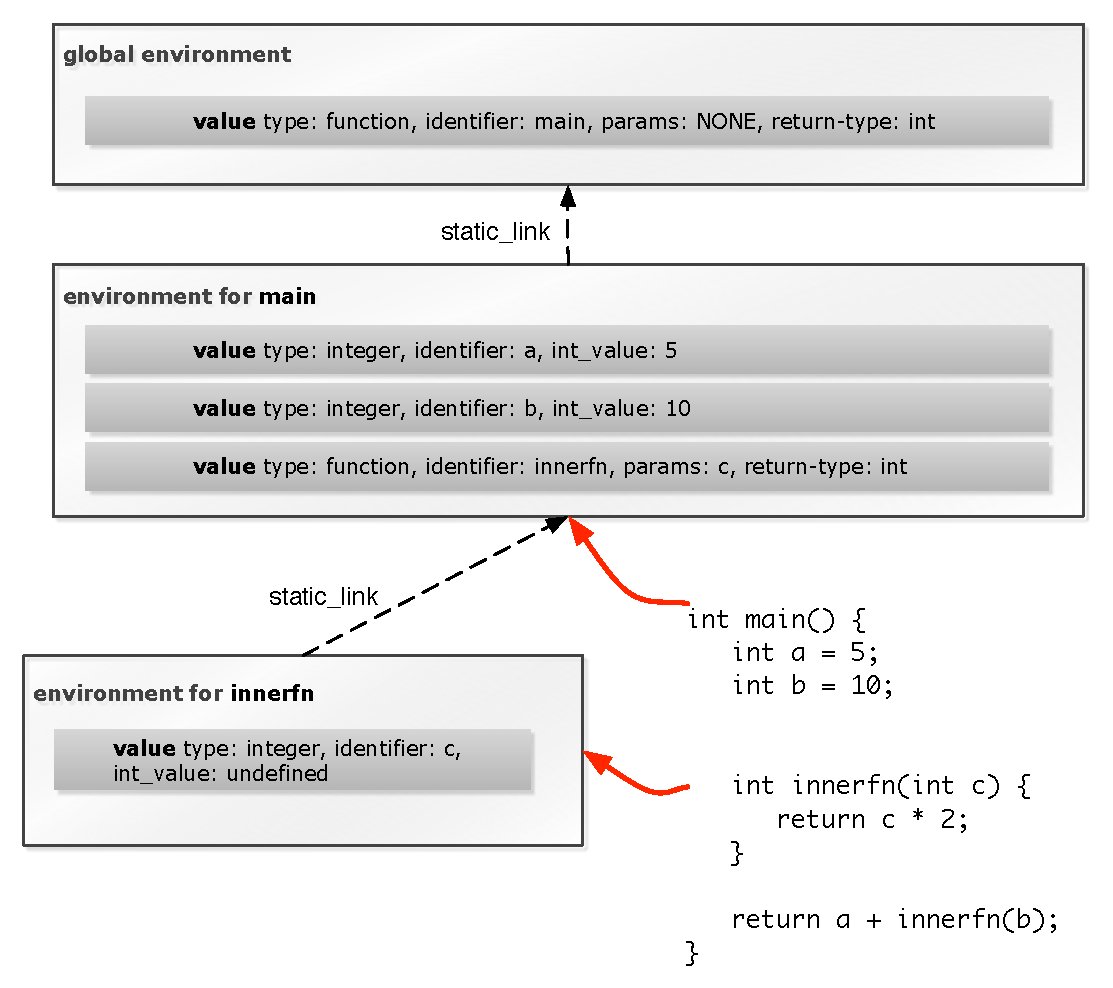
\includegraphics[scale=0.7]{environments-include.pdf}
	\caption{Environment Layout - Environment $\rightarrow$ Code relationship}
	\label{fig:environment}	
\end{figure}

\begin{figure}[p]
	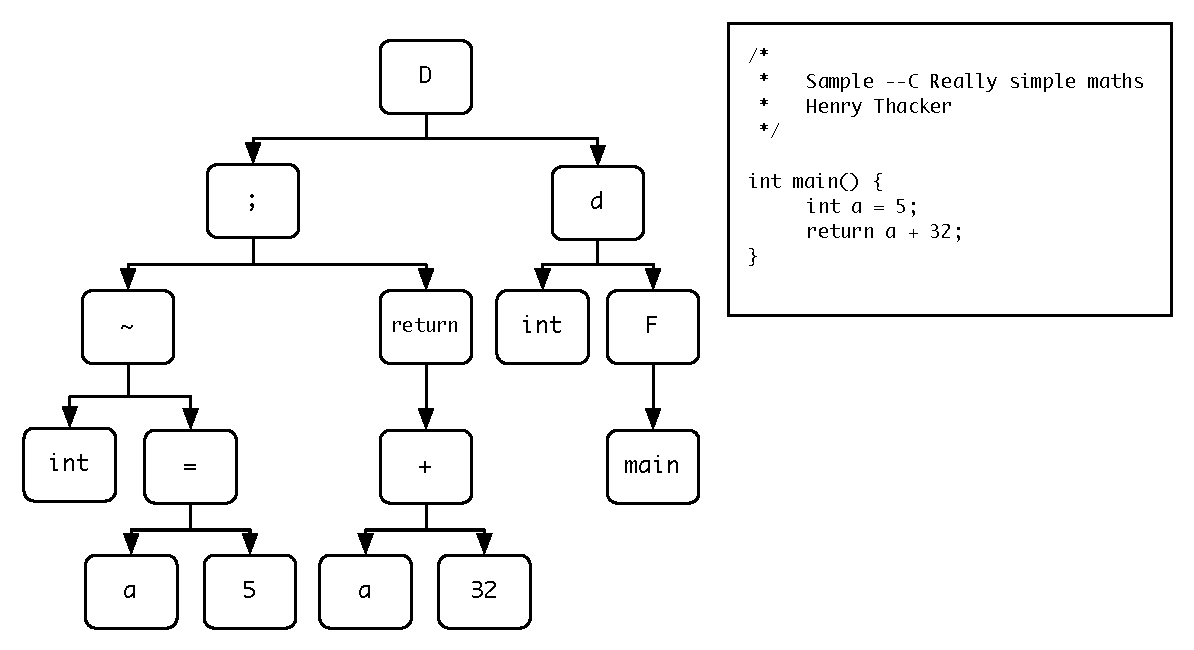
\includegraphics[scale=0.7]{ast-include.pdf}
	\caption{Abstract syntax tree example}
	\label{fig:ast}
\end{figure}

\begin{figure}[p]
	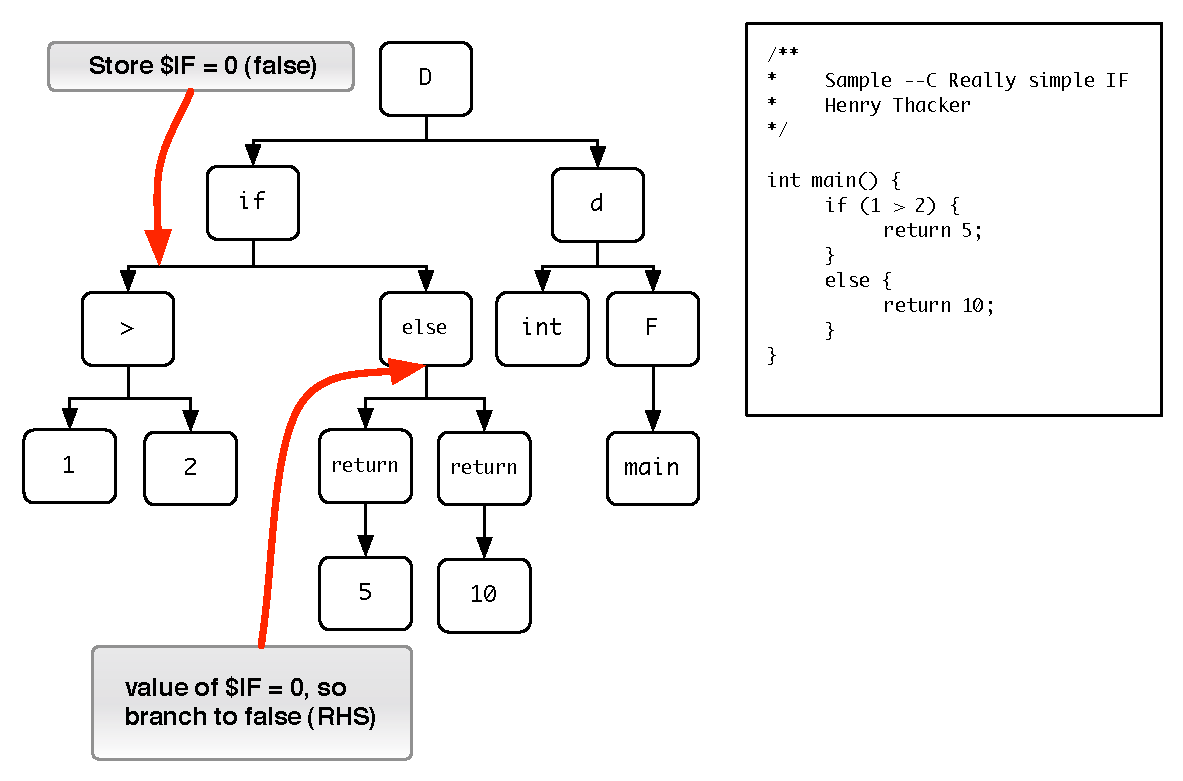
\includegraphics[scale=0.7]{if-include.pdf}
	\caption{IF, ELSE example}
	\label{fig:if}
\end{figure}

\begin{figure}[p]
	\begin{verbatim}
		typedef struct tac_quad {
		    char *op; /* Operation, i.e. + for addition */
		    value *operand1; /* A ptr to the first operand, could be an integer A */
		    value *operand2  /* A ptr to the first operand, could be an integer B */
		    value *result; /* The ptr to where the result will be stored, C */
		    int type; /* TT_OP - The type is an (arithmetic) operation */
		    int subtype; /* Reserved for categorisation of more granular operations */
		    int level; /* Used for MIPS code generation */
		    struct tac_quad *next; /* Pointer to the next tac_quad */		
		}tac_quad;
	\end{verbatim}
	\caption{tac\_quad structure}
	\label{fig:tacquad}
\end{figure}

\section{Intermediate Representation}

\subsection{Introduction}
In the coursework specification we were asked to develop a three address code representation of our own design. The input to the Three Address Code generator is the AST (\emph{Abstract Syntax tree}). The coursework specification indicates that it should be possible to read TAC (\emph{Three Address Code}) from a flat file. This was not implemented due to time pressures and it was felt that it was more important to move onto code generation, rather than write a TAC parser. The next section \ref{sec:tacintro} presents further background information behind the rationale of using a form of intermediate representation and the associated design choices that were made.

\subsection{Relation to the Interpreter}
The TAC is generated in a very similar way to how the interpreter works, using a large recursive function which handles all the different types of \verb!NODE!. Instead of evaluating the result of operations, we are interested in building TAC ``quadruples", internally referred to as a \verb!tac_quad!. Each \verb!tac_quad! is one TAC instruction and contains a \textbf{maximum} of three addresses (operand1, operand2, result) and several other pieces of metadata (please see figure \ref{fig:tacquad}). A \verb!tac_quad! does not contain text or lexemes, each address points to a \verb!value! within our environment. Thus, we are able to perform type checking and environment traversal, just as the interpreter does. The TAC generator generates a linked list of these \verb!tac_quad!s that represent the user-supplied \mmc source.
\ \\ \ \\
As with the interpreter, a pre-scan is done to find all globally accessible functions. All of the global functions which are found are entered into the global environment. We have to perform this pre-scan, because when we look up function names, we must be able to point our \verb!tac_quad!s to the correct references within the relevant environment. No notion of an entry-point is required during TAC generation, because the AST is traversed in its entirety from top to bottom, generating \verb!tac_quad!s on the fly. Unlike the interpreter, global variables are not found in the pre-scan, as this can be done as part of the main scan mentioned below.

\subsection{Temporaries} \label{sec:temporaries}
In Three Address Code, we are limited to a \textbf{maximum} of three addresses. Obviously, we cannot expect to complete any given operation in such a limited space, i.e. : $a = 1 + 3 + 2 + 10$ (4 operations, 5 addresses). In lectures, we were introduced to the concept of temporaries. We can assume that we have an infinite number of temporaries, but they must only appear on the LHS of an expression once. This allows us to split up complex expressions into ``\textbf{simple}" subexpressions stored in temporaries, that can be combined. This ``making simple" procedure is important in the implementation. Thus, our previous example becomes written as a series of simple instructions, seen in listing \ref{lst:temporaries}.
\ \\
\begin{lstlisting}[showstringspaces=false,language=java,breaklines=true, backgroundcolor=\color{light-gray}, captionpos=b, label={lst:temporaries}, caption={Using Temporaries}]
	_t1 = 1 + 3
	_t2 = 2 + 10
	a = _t1 + _t2
\end{lstlisting}
\ \\ \ \\
In the TAC Generator implementation, temporaries are embraced as full members of the environment. Temporaries are not treated any differently from variables and are accessed using the same functions. 

\subsection{Building tac\_quads}
After we have completed the pre-scan to populate our global environment, a full scan is made starting from the top of the AST. The TAC instructions are formed by examining each \verb!NODE! and evaluating the LHS and RHS until we have enough information to form a single, complete TAC instruction. The concept of ``make simple" was introduced in section \ref{sec:temporaries} and it refers to the process of reducing complex expressions to a temporary (i.e. the simplest form possible). Our recursive function in the TAC generator is actually called \verb!make_simple! and at each stage, it tries to reduce a subexpression to the simplest form it can (often a temporary). The steps that are taken for a few different \verb!NODE! types are given below.

\begin{description}
	\item[Arithmetic Operator] An integer temporary is created in preparation to hold to results of the arithmetic expression. The LHS and RHS of the operator are passed recursively to \verb!make_simple! to coerce them into integers. If the LHS or RHS are not simple integers or variables, they may themselves be made into integer temporaries. A call is made to \verb!make_quad_value! to build a \verb!tac_quad! of type \verb!TT_OP! (TAC type operation). Operands 1 and 2 are set to reference the LHS and RHS \verb!value!s that were returned by the calls to \verb!make_simple!. The result member of \verb!tac_quad! is set to reference the temporary that we created earlier to hold the result. The resultant \verb!tac_quad! is written into the linked list of TAC statements generated so far.
	\item[= Operator] Both the LHS (assignment variable) and RHS (assignment value) are passed to \verb!make_simple!. The current environment is searched to ensure that the assignment variable has already been defined, if not, an error is raised. During simplification, the RHS will be reduced to a simple constant, variable or temporary. The simplified value can then be type checked against the declaration for the assignment variable, to ensure that the assignment is valid. If so, the assignment is made in the environment. A \verb!tac_quad! is generated of type \verb!TT_ASSIGN!, an operation of ``$=$", operand 1 is set to reference the assignment value and result is set to reference the assignment variable. The \verb!tac_quad! is added to our list of existing \verb!tac_quad!s.
	\item[APPLY] Again, the LHS and RHS of the AST are passed to \verb!make_simple!. The LHS contains the function name, while the RHS contains the list of actual parameters to be passed to the function. The environment is searched to check that a function by this name exists in local scope. If the function can not be found an error is raised. Prior to making the actual function call, a few different TAC quads are created to assist during the code generation stage. Firstly a ``prepare to call" (\verb!TT_PREPARE!) quad is created with a reference to the function (please see the next chapter for the syntax), to instruct that a function call is about to be made. Next, the actual parameters list (RHS) is passed to another recursive function which generates push statements (\verb!TT_PUSH_PARAM!) for each parameter in the \textbf{reverse order} of their definition. This was decided after reading a technique mentioned in ``Modern Compiler Design"\cite{grune2000}: ``When parameters are passed on the stack, the last parameter is pushed first".
\\ \ \\ \
From the function definition found in the environment, we see if a return type was defined. A return type may not be available if the function is a function typed variable, as this will only be bound to another function at runtime. If a return type was found, we create an appropriately-typed temporary in which to store the result of the function application. If no return type was available, a typeless temporary is created. A \verb!TT_FN_CALL! \verb!tac_quad! is generated with a reference to the function definition stored in the operand1 member and a reference to our return value temporary in the result member. The created ``result temporary" is returned as the result of the \verb!make_simple! call, so that the function's result can be used in other expressions. 
	\item[IF and ELSE] On the LHS of an \verb!IF! statement is the condition. The condition is passed to \verb!make_simple! to simplify it to a single term. A TAC goto statement is generated that is jumped to in the event of the condition being true. The label name is automatically generated as \verb!__ifXtrue! (where $X$ is an integer which increments for each \verb!IF! statement that is created). The actual label itself will be defined later on.
\\ \ \\ \
The node on the RHS is examined to see if it is an \verb!ELSE! statement. If it is, we call \verb!make_simple! on the RHS (the false portion) and append the TAC that was created. After the false branch we create a jump to the end of the \verb!IF! statement with a similar label that will be defined later on: \verb!__ifXend!. 
\\ \ \\ \
In both cases (with and without an \verb!ELSE!) the true portion of the \verb!IF! statement is now translated. We generate a \verb!TT_LABEL! denoting the start of the true section (as we discussed earlier: \verb!__ifXtrue!). The true branch is now passed to \verb!make_simple!. Finally, to complete the \verb!IF! statement, the aforementioned end label is appended.
	\item[WHILE] While statements are rewritten as \verb!IF! statements, but with a jump back to the condition at the end of the true branch.
	\item[Functions] Each function declaration generates a minimum of 5 TAC instructions, these are detailed in the relevant sections below. It may help to look at figures \ref{fig:printedtac} and \ref{fig:ast} in addition to the textual description.
		\begin{description}
			\item[D] The LHS is passed to \verb!make_simple!. This yields a basic \verb!VT_FUNCTN! value which, by this stage, contains much of the required information regarding the function's definition. This function definition is stored in the environment. Several TAC statements are now generated, the semantics of these statements should be referred to in the next section (section \ref{sec:tacintro}).
\\ \ \\ \
Firstly a \verb!TT_BEGIN_FN! is created, with operand1 set to the function reference. Immediately after this, a \verb!TT_FN_DEF! \verb!tac_quad! is created, again with a reference to the function kept in its operand1 member. \verb!TT_FN_DEF! is used to print out the start of function label in the code generator. Next, a \verb!TT_INIT_FRAME! quad is created, with zero entered as operand1. \verb!TT_INIT_FRAME! gives important information about the required frame size (see section \ref{sec:MIPS}) to the code generation stage. However, at this point in the TAC generator, we do not know how large the frame needs to be, until we call \verb!make_simple! on the function body so that the environment becomes filled. By adding a placeholder in the correct place, but with a dummy value, it is possible  to return to this statement and fill in the correct frame size, when it is eventually known.
\ \\ \ \\
Next, the \textbf{formal} parameters are each popped off in \verb!TT_POP_PARAM! operations in the \textbf{order that they were defined}. Because the parameters are pushed to \textbf{function calls} in reverse order (see the description of \verb!APPLY! above), we now assume we can read the actual parameters off some type of virtual argument stack, which are now conveniently accessible in the correct order. Each parameter is given a dummy value (0, null, etc.) depending on the parameter type and stored as a regular variable in the environment. Thus, each \verb!TT_POP_PARAM! references the relevant uninitialised variable within the function's environment. To mark the end of parameters and the start of user-supplied code, we append a \verb!TT_FN_BODY! \verb!tac_quad!. Now \verb!make_simple! is called on the RHS (function body).
\ \\ \ \\
After all TAC has been generated for the function body, we can query the size of the final environment, using a utility function \verb!env_size!. The previously created \verb!TT_INIT_FRAME! quad is updated with the correct value. Finally, a \verb!TT_END_FN! instruction is created to denote the end of the function.
			\item[d, F] No TAC instructions are generated here, but a \verb!VT_FUNCTN! \verb!value! is built to pass up to the \verb!D! node. The procedure here is exactly the same as with the interpreter.
		\end{description}
	\item[RETURN] For a return statement, if the LHS is not null, it is passed to \verb!make_simple!. If the LHS is an identifier, then this identifier is searched for in the environment. Identifiers may appear on the LHS if the function returns a function or integer-typed variable, for instance. A type check is performed on the return value to ensure it is consistent with the function definition. We now append a \verb!TT_RETURN! \verb!tac_quad! and set the operand1 member to the returned value (or null for a void function).
\end{description}

\subsection{Output of tac\_quads}
By the time the \verb!make_simple! call returns, a linked list of complete \verb!tac_quad! structures has been created that constitutes the translation of the user \mmc program into TAC representation. As mentioned previously, these structures do not contain strings or lexemes, but contain pointers in to an environment structure. Originally the \verb!tac_quad! \textbf{did} simply store the lexemes instead of pointers, but the code was refactored after reading several texts and consulting the lecturers. One major source of reference was the course text which summed up the correct path to take.
\begin{quotation}
	\ \\
	``In an implementation [of Three Address Code quads], a source name is replaced by a pointer to its symbol-table entry, where all information about the name is kept." \cite{aho2007}.
\end{quotation}
\ \\
When thinking \emph{purely} about Three Address Code, it is hard to see why pointers into the environment are required at all. In fact, this information does not appear to even be mentioned in the various texts. This is why the \verb!tac_quad!s were originally designed (incorrectly) to use lexemes instead. However, it quickly became clear that because the TAC will be passed into the code-generator, it is useful to have access to scope information (provided by the environment structure already) and the type checking routines that are also available. As well as reducing the code outlay, the environment code was rigorously tested as part of the interpreter.
\ \\ \ \\
Up until now, the description of the recursive function \verb!make_simple! has mentioned \verb!NODE! types such as \verb!TT_OP!, \verb!TT_LABEL! etc. This view onto TAC instructions is the way that the TAC generator internally builds and examines the TAC, additionally an optimiser or code-generator would also choose to look at the TAC quads in this fashion. However, as humans, looking at a list of opcodes and pointers is not intuitive, thus a printable TAC representation is created from the instructions with the supplied \verb!print_tac! function (an example is given in figure \ref{fig:printedtac}). Had a TAC parser been implemented (to load TAC from a file, populating the environment), this would also have been the required input language (discussed further in \ref{sec:tacintro}). The \verb!print_tac! function understands the syntax and semantics of the TAC language and is able to print out any given TAC instruction.
\ \\ \ \\
\verb!print_tac! is another recursive function that walks over the list of generated \verb!tac_node!s and writes out the ``human readable" form of each quad. The rewrite rules for each TAC operation are given below.
\begin{description}
	\item[TT\_LABEL] 
\end{description}

\begin{figure}[p]
	\begin{verbatim}
		/** 
		 * Please note the indentation/spacing/comments below are NOT present in the
		 * generated TAC, but are introduced here to improve legibility
		 **/

		/* cplus function */
		
		BeginFn cplus
		_cplus:
		InitFrame 2
		PopParam a
		FnBody
		
		   /* Inner function cplusa */
		   BeginFn cplusa
		   _cplusa:
		   InitFrame 2
		   PopParam b
		   FnBody
		      _t1 = a + b
		      Return _t1
		   EndFn
		
		Return cplusa
		EndFn
		
		/* Main function */
		
		BeginFn main
		_main:
		InitFrame 4
		FnBody
		   PrepareToCall 1
		   PushParam 5
		   _t2 = CallFn _cplus
		   z = _t2
		   PrepareToCall 1
		   PushParam 9
		   _t3 = CallFn _z
		   Return _t3
		EndFn

		
	\end{verbatim}
	\caption{Printed TAC output}
	\label{fig:printedtac}
\end{figure}

\subsection{Machine Independent Optimisation (MIO)}
\label{sec:MIO}

\subsection{State of the TAC Generator}
The TAC generator is perhaps a slightly smaller part of this project than was intended by the coursework specification. It \textbf{is} a module in its own right and can be run independently of the code generator. However, it requires input from the parser to function. Unfortunately there was no time to implement a separate TAC parser, although this will be discussed in the Critical Evaluation section in further detail.
\\ \ \\ \
Functionally, the TAC generator is not \emph{as} complete as the interpreter, but it is still able to execute almost all of the examples as intended. One area that is lacking is the creation of new environments within \verb!IF! and \verb!WHILE! statements. This means that the behaviour when redefining an existing variable has not been rigorously tested and is likely to break.
\\ \ \\ \
Additionally as mentioned in the section on Machine Independent Optimisation (section \ref{sec:MIO}), there was simply no time to investigate various optimisations that could have been put to use. This, again, is covered in further detail in the Critical Evaluation section.
\section{MIPS Assembler Compiler}
\label{sec:MIPS}